\documentclass[a4paper, 10pt, conference]{ieeeconf}
\IEEEoverridecommandlockouts
\overrideIEEEmargins
\usepackage{listings}
\usepackage[dvipsnames]{xcolor}
\usepackage{graphicx}

\renewcommand\thesection{\arabic{section}}
%\renewcommand\thesubsection{\thesection.\arabic{subsection}}


\title{\LARGE \bf F2FS and EXT4 Reliability}
\author{Michael Meerbott}

\lstset{ %
    language=c,
    backgroundcolor=\color{white},   % choose the background color
    basicstyle=\footnotesize,        % size of fonts used for the code
    breaklines=true,                 % automatic line breaking only at whitesp
    captionpos=b,                    % sets the caption-position to bottom
    commentstyle=\color{Brown},    % comment style
    keywordstyle=\color{blue},       % keyword style
    stringstyle=\color{RedViolet},     % string literal style
    showstringspaces=false,
    frame=lrtb,
    columns=fullflexible,
}

\begin{document}
\maketitle
\thispagestyle{empty}
\pagestyle{empty}

%%%%%%%%%%%%%%%%%%%%%%%%%%%%%%%%%%%%%%%%%%%%%%%%%%%%%%%%%%%%%%%%%%%%%%%%%%%%%%%%
\section*{Abstract}
Flash storage is becoming more prevalent in user level devices. Today, the 
Android operating system defaults to using EXT4 as its default filesystem, as 
do many Linux distributions. Most mobile phones use NAND flash storage devices
and many lapotps today are using the same. F2FS was created by Samsung to 
take advantage of the NAND flash structure to optimize speeds \cite{c0}. 
In this project, I wanted to compare the reliability of F2FS to that of EXT4 to
help people, including myself, decide if it is worth the risk to switch 
their flash storage systems over to F2FS. I age both EXT4 and F2FS and show 
that F2FS does not seem to outperform EXT4.

%%%%%%%%%%%%%%%%%%%%%%%%%%%%%%%%%%%%%%%%%%%%%%%%%%%%%%%%%%%%%%%%%%%%%%%%%%%%%%%%
\section{INTRODUCTION}
Over time, filesystems may operate slow due to file fragmentation. Filesystem
aging is the measure of fragmentation over time. In this project, I use the
aging method from the paper ``File Systems Fated for Senescence? Nonsense, 
Says Science!" by A. Conway et al. \cite{c1}. The method uses a sequence of 
Git pulls of the Linux source code onto a device. After a number of pulls, it 
then performs a grep test. The grep test simply performs a grep of a 
non-existing string on the root directory of the source code and times how long
the grep takes. It then continues on, creating a timeline of grep times after
a total number of pulls. 

\section{Methodology}
\subsection*{System Setup}
The project was performed on a ThinkPad E330 running Ubuntu 16.04.5 (Linux
4.4.0-104-generic). The tools for F2FS used, F2FS-tools mkfs-f2fs, was 1.6.1.
The filesystems were aged on a 32 GB SanDisk Ultra class 10 SD 
card that was split evenly into 4 partitions of 7.43 GB each. The 
card used 2 partitions of F2FS and 2 partitions of EXT4. Both filesystems use
one partition for aging and one ``clean" partition to compare the aging against.
Below are the configurations I used to create the filesystems, which are 
the defaults:
\\[10pt]
F2FS
\lstinputlisting{options_f2fs}
EXT4
\lstinputlisting{options_ext4}

\subsection*{Git Pull Configurations}
There are 2 configurations used for the git pull aging. The first
tests run 10,000 pulls and perform grep tests every 100 pulls. 
The second set runs 5,000 pulls and perform grep tests every 50 pulls.

\section{Issues and Difficulties}
The git-pull script was simple to set up, but didn't run as smoothly as hoped. 
After around 200 git pulls, the script would crash on a git pull with error
128. I re-ran the script several times with the first set of parameters.
I looked around online for error 128, but the search results were not 
consistent. Many of the search results were project specific (a project 
unrelated to what I was doing), and the others were mentioning a bad git ssh 
key, which was not my issue. The script would stop running after the first 
error, so I decided to simply insert a try-except block to see if the script
would continue immediately after the first error. I let it run for a few days, 
and when I checked the results, the script had not continued after the error
immediately, but instead after many more errors, and would fail again. It was
constantly off and on. I ran it 3 times with the 10,000-pulls setting to make
sure it would keep running with occasional results, and it seemed they were 
all at random pulls. 

I decided 10,000 runs was going to take too long with too little results, so I
reduced the tests to 5,000 pulls and grep tests after every 50 pulls. I ran
the script again for a few days for both filsystems, but the results did not 
show any notable aging, so I ran them again: 1 week for the F2FS tests and 1 
week for the EXT4 tests. Those are the results use in this report. 

\section{Results}
These results do not have a constant step size between the grep tests. This
is due to the failed git pulls, so I only added the pulls that succeeded. In 
Figure 1, we see that F2FS shows some aging after 250 git pulls. At the last
grep test (393 pulls), the results show the aged partition is about 1.14x 
slower than the unaged partition. Note that
the line should be compared with the non-aged line as a jump in Grep Cost can
mean an increase in number of files. The results also show some "free play" 
range: in the initial pull, both partitions are clean and unaged, yet we see
a difference of .677 sec/GB in the grep cost.

Figure 2 shows our results for EXT4. These results do not show any aging, 
since the difference between all of the points is close to the "free play" we
see on the initial test. The difference in the initial test is .481 sec/GB. 
These results tell us that EXT4 is more reliable in terms of aging than F2FS
since it showed less aging.

Figure 3 compares the F2FS and EXT4 results against each other. Surprisingly,
the initial EXT4 results outperform F2FS by around 50\% (EXT4 is 1.5x faster).
SD cards use NAND flash storage, so F2FS was expected to run faster. I am not
sure why EXT4 outperformed F2FS; it could be the version of f2fs-tools I used,
or the version of Linux I used. 

Overall, I would say that these results are inconclusive. There is not enough
data/git-pulls to decide anything. For conclusive results, I would expect to 
see some obvious EXT4 aging. The fact that EXT4 immediately outperformed F2FS
is also odd, especially since most speed tests show F2FS performing better. 


\section{Future Work}

I would recommend using more than one aging tool for this and testing it on different
storage devices or systems since my laptop had EXT4 always outperforming F2FS. A variety of
methods should also be considered, since the script used goes by commits in one project.
This would have a limited number of changes per commit pulled. This may not provide enough
data changes for aging the filesystem.

%F2FS
\begin{figure}
	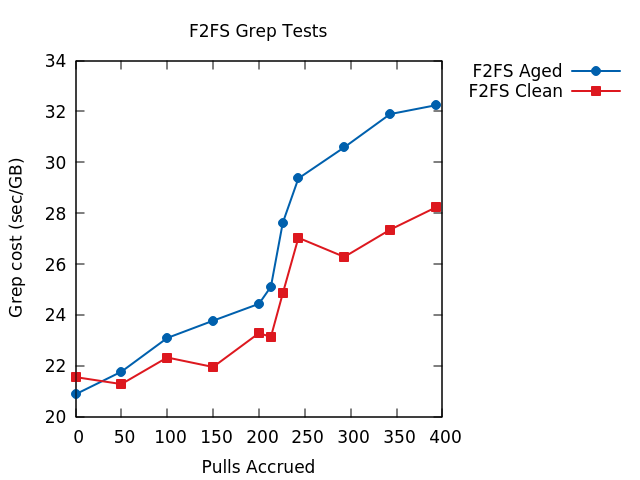
\includegraphics[width=\linewidth]{f2fs_aged.png}
	\caption{The F2FS results with aged and unaged tests}
	\label{fig:f2fs}
\end{figure}

%EXT4
\begin{figure}
	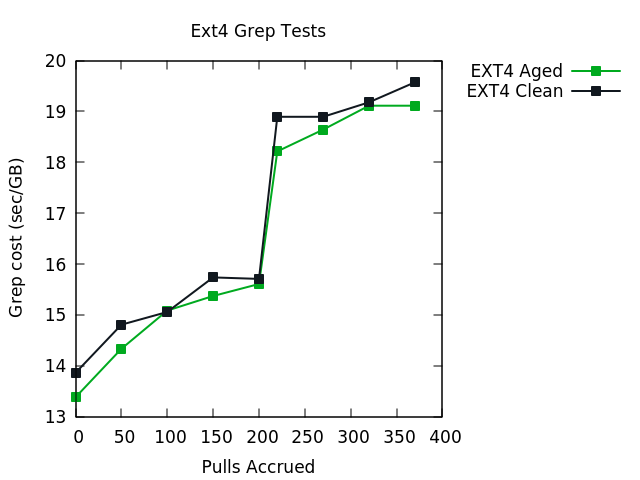
\includegraphics[width=\linewidth]{ext4_aged.png}
	\caption{The EXT4 results with aged and unaged tests}
	\label{fig:f2fs}
\end{figure}

%BOTH
\begin{figure}
	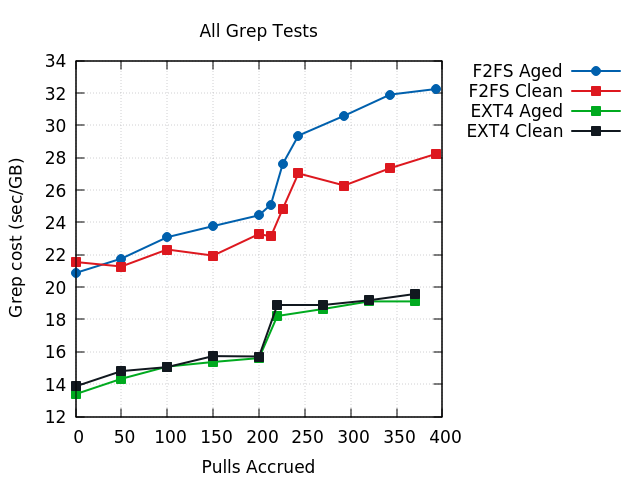
\includegraphics[width=\linewidth]{All.png}
	\caption{Both F2FS and EXT4 (aged and unaged) results compared}
	\label{fig:f2fs}
\end{figure}



\addtolength{\textheight}{-12cm}   % This do balance the column lengths
%%%%%%%%%%%%%%%%%%%%%%%%%%%%%%%%%%%%%%%%%%%%%%%%%%%%%%%%%%%%%%%%%%%%%%%%%%%%%%%%



\begin{thebibliography}{99}

\bibitem{c0} Changman Lee, Dongho Sim, Joo-Young Hwang, and Sangyeun Cho. 2015. F2FS: a new file system for flash storage. In Proceedings of the 13th USENIX Conference on File and Storage Technologies (FAST'15). USENIX Association, Berkeley, CA, USA, 273-286.

\bibitem{c1} Alex Conway, Ainesh Bakshi, Yizheng Jiao, Yang Zhan, Michael A. Bender, William Jannen, Rob Johnson, Bradley C. Kuszmaul, Donald E. Porter, Jun Yuan, and Martin Farach-Colton. 2017. File systems fated for senescence? nonsense, says science!. In Proceedings of the 15th Usenix Conference on File and Storage Technologies (FAST'17). USENIX Association, Berkeley, CA, USA, 45-58

\end{thebibliography}

\end{document}

